\tikzset{every picture/.style={line width=0.75pt}} %set default line width to 0.75pt        

% \begin{scaletikzpicturetowidth}{\textwidth}
% \begin{tikzpicture}[scale=\tikzscale]
\begin{tikzpicture}[x=0.75pt,y=0.75pt,yscale=-1.5,xscale=1.5]
%uncomment if require: \path (0,682); %set diagram left start at 0, and has height of 682

%Shape: Path Data [id:dp5167310974654173] 
\draw   (192.73,91.34) -- (192.54,125.45) -- (157.65,135.4) -- (157.94,81.08) -- (192.73,91.34) -- cycle (203.86,125.3) -- (204.05,91.19) -- (238.95,81.23) -- (238.65,135.56) -- (203.86,125.3) -- cycle ;
%Image [id:dp6554124786483229] 
\draw (97.9,110.28) node  {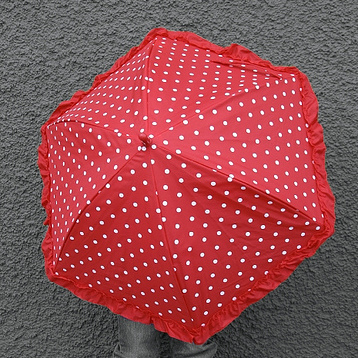
\includegraphics[scale=0.2]{figures/multiprox/noisy_image_0.jpg}};
%Image [id:dp6114334376607021] 
\draw (621.88,107) node  {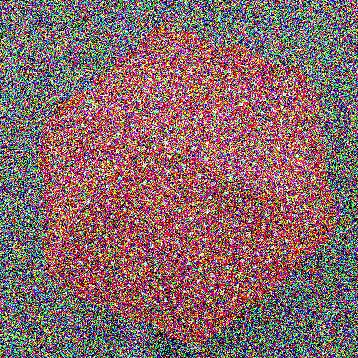
\includegraphics[scale=0.2]{figures/multiprox/noisy_image_200.jpg}};
%Shape: Path Data [id:dp6505449591813888] 
\draw   (519.2,94.47) -- (519.04,124.36) -- (490.26,133.09) -- (490.51,85.48) -- (519.2,94.47) -- cycle (528.38,124.23) -- (528.53,94.34) -- (557.31,85.62) -- (557.07,133.22) -- (528.38,124.23) -- cycle ;
%Image [id:dp2887609865363622] 
\draw (803.7,104.43) node  {
\includegraphics[scale=0.2]{figures/multiprox/noisy_image_1000.jpg}};
%Image [id:dp06399820414495216] 
\draw (299.23,107.27) node  {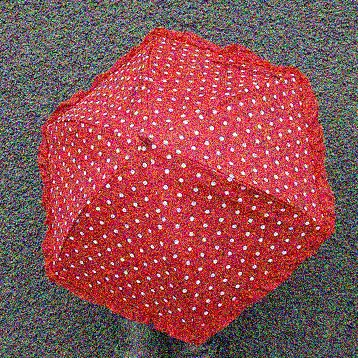
\includegraphics[scale=0.2]{figures/multiprox/noisy_image_50.jpg}};
%Shape: Path Data [id:dp35904403541774765] 
\draw   (706.89,88.33) -- (706.7,122.44) -- (671.8,132.39) -- (672.1,78.07) -- (706.89,88.33) -- cycle (718.02,122.29) -- (718.21,88.18) -- (753.1,78.22) -- (752.81,132.55) -- (718.02,122.29) -- cycle ;
%Straight Lines [id:da22795902524183642] 
\draw    (56.73,178.36) -- (843.14,179.61) ;
%Image [id:dp8635213845314278] 
\draw (130.83,441.89) node  {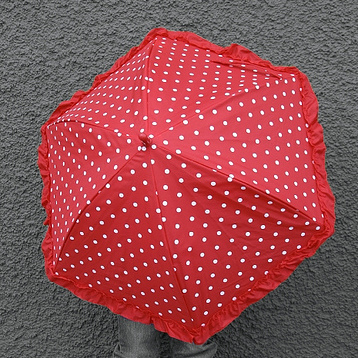
\includegraphics[scale=0.2]{figures/multiprox/noisy_image_0.jpg}};
%Image [id:dp010023251321917837] 
\draw (675.11,361.08) node  {
\includegraphics[scale=0.13]{figures/multiprox/noisy_image_1000.jpg}};
%Curve Lines [id:da4369376972969814] 
\draw    (652.11,366.71) .. controls (595.94,355.93) and (551.78,380.01) .. (519.25,409.75) ;
\draw [shift={(518.27,410.66)}, rotate = 317.25] [color={rgb, 255:red, 0; green, 0; blue, 0 }  ][line width=0.75]    (10.93,-3.29) .. controls (6.95,-1.4) and (3.31,-0.3) .. (0,0) .. controls (3.31,0.3) and (6.95,1.4) .. (10.93,3.29)   ;
%Image [id:dp7607350242636655] 
\draw (420.81,437.92) node  {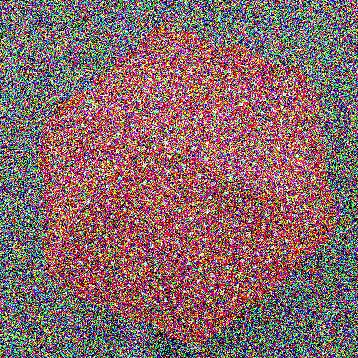
\includegraphics[scale=0.2]{figures/multiprox/noisy_image_200.jpg}};
%Curve Lines [id:da5154956030822916] 
\draw    (657.64,410.66) .. controls (589.7,387.94) and (545.71,413.43) .. (521.57,423.61) ;
\draw [shift={(519.75,424.37)}, rotate = 337.98] [color={rgb, 255:red, 0; green, 0; blue, 0 }  ][line width=0.75]    (10.93,-3.29) .. controls (6.95,-1.4) and (3.31,-0.3) .. (0,0) .. controls (3.31,0.3) and (6.95,1.4) .. (10.93,3.29)   ;
%Curve Lines [id:da9083922123678473] 
\draw    (651.71,518.95) .. controls (618.83,520.5) and (556.5,491.31) .. (522.04,470.79) ;
\draw [shift={(520.49,469.85)}, rotate = 31.09] [color={rgb, 255:red, 0; green, 0; blue, 0 }  ][line width=0.75]    (10.93,-3.29) .. controls (6.95,-1.4) and (3.31,-0.3) .. (0,0) .. controls (3.31,0.3) and (6.95,1.4) .. (10.93,3.29)   ;
%Curve Lines [id:da8748816234764569] 
\draw    (654.68,466.86) .. controls (583.48,480.3) and (548.59,455.79) .. (521.4,444.25) ;
\draw [shift={(519.75,443.56)}, rotate = 22.24] [color={rgb, 255:red, 0; green, 0; blue, 0 }  ][line width=0.75]    (10.93,-3.29) .. controls (6.95,-1.4) and (3.31,-0.3) .. (0,0) .. controls (3.31,0.3) and (6.95,1.4) .. (10.93,3.29)   ;
%Curve Lines [id:da40366686687455766] 
\draw    (703.13,359.77) .. controls (724.34,384.3) and (715.26,392.39) .. (706.7,406.25) ;
\draw [shift={(705.77,407.78)}, rotate = 300.66] [color={rgb, 255:red, 0; green, 0; blue, 0 }  ][line width=0.75]    (10.93,-3.29) .. controls (6.95,-1.4) and (3.31,-0.3) .. (0,0) .. controls (3.31,0.3) and (6.95,1.4) .. (10.93,3.29)   ;
%Curve Lines [id:da046176827312971236] 
\draw    (703.43,416.86) .. controls (724.63,441.39) and (715.55,449.48) .. (706.99,463.34) ;
\draw [shift={(706.06,464.87)}, rotate = 300.66] [color={rgb, 255:red, 0; green, 0; blue, 0 }  ][line width=0.75]    (10.93,-3.29) .. controls (6.95,-1.4) and (3.31,-0.3) .. (0,0) .. controls (3.31,0.3) and (6.95,1.4) .. (10.93,3.29)   ;
%Curve Lines [id:da11631948476544929] 
\draw    (703.92,477.8) .. controls (725.12,502.33) and (716.04,510.42) .. (707.48,524.28) ;
\draw [shift={(706.55,525.81)}, rotate = 300.66] [color={rgb, 255:red, 0; green, 0; blue, 0 }  ][line width=0.75]    (10.93,-3.29) .. controls (6.95,-1.4) and (3.31,-0.3) .. (0,0) .. controls (3.31,0.3) and (6.95,1.4) .. (10.93,3.29)   ;
%Shape: Path Data [id:dp27188545151292254] 
\draw   (264.39,422.51) -- (264.2,456.24) -- (228.76,466.08) -- (229.06,412.37) -- (264.39,422.51) -- cycle (275.69,456.09) -- (275.88,422.36) -- (311.32,412.52) -- (311.02,466.23) -- (275.69,456.09) -- cycle ;
%Shape: Path Data [id:dp4703662550452038] 
\draw   (393.45,94.57) -- (393.29,124.8) -- (364.01,133.62) -- (364.25,85.48) -- (393.45,94.57) -- cycle (402.79,124.66) -- (402.95,94.44) -- (432.24,85.62) -- (431.99,133.75) -- (402.79,124.66) -- cycle ;
%Image [id:dp31284811925683054] 
\draw (675.11,413.18) node  {
\includegraphics[scale=0.13]{figures/multiprox/noisy_image_1000.jpg}};
%Image [id:dp5047856851088827] 
\draw (676.16,465.48) node  {
\includegraphics[scale=0.13]{figures/multiprox/noisy_image_1000.jpg}};
%Image [id:dp847963556826254] 
\draw (676.16,518.94) node  {
\includegraphics[scale=0.13]{figures/multiprox/noisy_image_1000.jpg}};

% Text Node
\draw (154.13,143.22) node [anchor=north west][inner sep=0.75pt]  [font=\small] [align=left] {{\small Denoising U-net}};
% Text Node
\draw (672.69,142.05) node [anchor=north west][inner sep=0.75pt]  [font=\footnotesize] [align=left] {Denoising U-net};
% Text Node
\draw (379.67,306.74) node [anchor=north west][inner sep=0.75pt]  [font=\Large,color={rgb, 255:red, 139; green, 87; blue, 42 }  ,opacity=1 ] [align=left] {{\large {\fontfamily{pcr}\selectfont \textbf{Averaging}}}};
% Text Node
\draw (179.98,483.98) node [anchor=north west][inner sep=0.75pt]   [align=left] {{\fontfamily{pcr}\selectfont \textbf{\textcolor[rgb]{0.96,0.65,0.14}{{\large Denoise with a RGO}}}}};
% Text Node
\draw (766.52,405.84) node [anchor=north west][inner sep=0.75pt]   [align=left] {\textbf{\textcolor[rgb]{0.25,0.46,0.02}{Gibbs Sampling}}};
% Text Node
\draw (446.22,90.88) node [anchor=north west][inner sep=0.75pt]   [align=left] {\textbf{{\large ...}}};
% Text Node
\draw (377.95,143.97) node [anchor=north west][inner sep=0.75pt]  [font=\small] [align=left] {{\small Sequence of Denoising U-nets}};
% Text Node
\draw (589.06,282.25) node [anchor=north west][inner sep=0.75pt]    {${\displaystyle Y_{i} =\ e^{-t} X\ +\ \sqrt{1-e^{-2t}} \ Z_{i}}$};
% Text Node
\draw (800.44,434.3) node [anchor=north west][inner sep=0.75pt]    {$Y_{i} |Y_{-i}$};
% Text Node
\draw (588.61,259.75) node [anchor=north west][inner sep=0.75pt]   [align=left] {{$m$ noisy measurements at a \textbf{fixed} $t$}};
% Text Node
% Text Node
\draw (321.78,339.39) node [anchor=north west][inner sep=0.75pt]  [font=\small]  {${\textstyle \frac{1}{m} \ \sum \ Y_{i}\overset{\mathcal{L}}{=} \ \ e^{-t} X\ +\ \sqrt{\frac{1\ -\ e^{-2t}}{m}} Z}$};
% Text Node
\draw (224.37,517.92) node [anchor=north west][inner sep=0.75pt]    {$X|Y_{1} \ \dotsc \ Y_{m}$};
% Text Node
\draw (295.16,12.08) node [anchor=north west][inner sep=0.75pt]   [align=left] {{\textbf{\textcolor[rgb]{0.61,0.61,0.61}{Classic Denoising diffusion framework}}}};
% Text Node
\draw (346.96,199.07) node [anchor=north west][inner sep=0.75pt]   [align=left] {{\fontfamily{pcr}\selectfont \textbf{{\large MultiProx Sampler}}}};
% Text Node
\draw  [color={rgb, 255:red, 65; green, 117; blue, 5 }  ,draw opacity=1 ][fill={rgb, 255:red, 65; green, 117; blue, 5 }  ,fill opacity=1 ]  (828.38, 490.62) circle [x radius= 20.88, y radius= 25.46]   ;
\draw (821.38,471.62) node [anchor=north west][inner sep=0.75pt]  [font=\LARGE,color={rgb, 255:red, 255; green, 255; blue, 255 }  ,opacity=1 ,xslant=0.24] [align=left] {A};
% Text Node
\draw  [color={rgb, 255:red, 245; green, 166; blue, 35 }  ,draw opacity=1 ][fill={rgb, 255:red, 245; green, 166; blue, 35 }  ,fill opacity=1 ]  (274.38, 572.62) circle [x radius= 22.73, y radius= 25.46]   ;
\draw (268.77,553.62) node [anchor=north west][inner sep=0.75pt]  [font=\LARGE,color={rgb, 255:red, 255; green, 255; blue, 255 }  ,opacity=1 ,xslant=0.31] [align=left] {B};
% Text Node
\begin{scope}[shift={(20pt, -45pt)}]
 % Rounded Rect 1 (Green) - Widened by 30pt + 20pt
    \draw  [color={rgb, 255:red, 65; green, 117; blue, 5 }  ,draw opacity=1 ][fill={rgb, 255:red, 65; green, 117; blue, 5 }  ,fill opacity=1 ]
           (914, 295.8) .. controls (914, 274.92) and (930.92, 258) .. (951.8, 258) --  % Left side x-coords -10pt
           (1258.2, 258) .. controls (1279.08, 258) and (1296, 274.92) .. (1296, 295.8) -- % Right side x-coords +10pt
           (1296, 409.2) .. controls (1296, 430.08) and (1279.08, 447) .. (1258.2, 447) -- % Right side x-coords +10pt
           (951.8, 447) .. controls (930.92, 447) and (914, 430.08) .. (914, 409.2) -- cycle ; % Left side x-coords -10pt

    % Rounded Rect 2 (Orange) - Widened by 30pt + 20pt
    \draw  [color={rgb, 255:red, 245; green, 166; blue, 35 }  ,draw opacity=1 ][fill={rgb, 255:red, 245; green, 166; blue, 35 }  ,fill opacity=1 ]
           (918, 510.8) .. controls (918, 489.92) and (934.92, 473) .. (955.8, 473) -- % Left side x-coords -10pt
           (1262.2, 473) .. controls (1283.08, 473) and (1300, 489.92) .. (1300, 510.8) -- % Right side x-coords +10pt
           (1300, 624.2) .. controls (1300, 645.08) and (1283.08, 662) .. (1262.2, 662) -- % Right side x-coords +10pt
           (955.8, 662) .. controls (934.92, 662) and (918, 645.08) .. (918, 624.2) -- cycle ; % Left side x-coords -10pt

    % Rounded Rect 3 (Gray/White) - Widened by 30pt + 20pt
    \draw  [color={rgb, 255:red, 255; green, 255; blue, 255 }  ,draw opacity=1 ][fill={rgb, 255:red, 155; green, 155; blue, 155 }  ,fill opacity=1 ]
           (919, 206) .. controls (919, 200.48) and (923.48, 196) .. (929, 196) -- % Left side x-coords -10pt
           (1282, 196) .. controls (1287.52, 196) and (1292, 200.48) .. (1292, 206) -- % Right side x-coords +10pt
           (1292, 236) .. controls (1292, 241.52) and (1287.52, 246) .. (1282, 246) -- % Right side x-coords +10pt
           (929, 246) .. controls (923.48, 246) and (919, 241.52) .. (919, 236) -- cycle ; % Left side x-coords -10pt
\end{scope}
\begin{scope}[shift={(-5pt, -45pt)}]
    
\draw (1012, 274) node [anchor=north west][inner sep=0.75pt]   [align=left] {{\Large \textbf{{\fontfamily{pcr}\selectfont \textcolor[rgb]{1,1,1}{Gibbs Sampling}}}}};
% Text Node
\draw (1018.44,380.3) node [anchor=north west][inner sep=0.75pt]  [color={rgb, 255:red, 255; green, 255; blue, 255 }  ,opacity=1 ]  {then\ $Y_{i} |Y_{-i}$ \ is\ log-concave.};
% Text Node
\draw (1024.5,321) node [anchor=north west][inner sep=0.75pt]  [color={rgb, 255:red, 255; green, 255; blue, 255 }  ,opacity=1 ]  {$If\ t\ \geq \ \cfrac{1}{2}\log\left( 1\ +\ \frac{L}{2}\right)$};
% Text Node
\draw (1040,491) node [anchor=north west][inner sep=0.75pt]   [align=left] {{\Large \textbf{{\fontfamily{pcr}\selectfont \textcolor[rgb]{1,1,1}{Denoising}}}}};
% Text Node
\draw (1012.5,537) node [anchor=north west][inner sep=0.75pt]  [font=\large,color={rgb, 255:red, 255; green, 255; blue, 255 }  ,opacity=1 ]  {$If\ m\ \geq \ 2\left( e^{2t} \ -\ 1\right) \ L$};
% Text Node
\draw (977.44,583.3) node [anchor=north west][inner sep=0.75pt]  [font=\large,color={rgb, 255:red, 255; green, 255; blue, 255 }  ,opacity=1 ]  {then\ $X|Y_{1} \dotsc Y_{m}$ \ is log-concave };
% Text Node
\draw (948,211) node [anchor=north west][inner sep=0.75pt] [align=left] {{ \textbf{{ \textcolor[rgb]{1,1,1}{Assumption:}}}}};
% Text Node
\draw (1108,211) node [anchor=north west][inner sep=0.75pt]  [color={rgb, 255:red, 255; green, 255; blue, 255 }  ,opacity=1 ]  {$\nabla \log p_X$  is $L$-Lipschitz.};
\end{scope}
\end{tikzpicture}
% \end{scaletikzpicturetowidth}